\documentclass[10pt]{beamer}
\usepackage[italian]{babel}
%\usepackage[utf8]{inputenc}

\usetheme{metropolis}
\usepackage{appendixnumberbeamer}

\usepackage{booktabs}
\usepackage[scale=2]{ccicons}

\usepackage{pgfplots}
\usepgfplotslibrary{dateplot}

\usepackage{listings}
\lstset{breaklines=true}

\usepackage{minted}

\usepackage{xspace}
\newcommand{\themename}{\textbf{\textsc{metropolis}}\xspace}

\title{Version Control systems and Git}
\subtitle{A brief introduction}
\date{\today}
\author{Enrico Bassetti}
\institute{Sapienza - University of Rome}
%\titlegraphic{\hfill\includegraphics[height=1.5cm]{.png}}

\begin{document}

\setbeamertemplate{frame footer}{Sapienza - University of Rome}

\maketitle

\begin{frame}{Roadmap}
  \setbeamertemplate{section in toc}[sections numbered]
  \tableofcontents[hideallsubsections]
\end{frame}


\section{Version control}

\begin{frame}[fragile]{Keeping track of versions}

Either alone or in a team, one big issue of software development is \textit{keeping
track of changes} on the source code.

\vspace{1em}

\textbf{Why?}
\begin{itemize}
\item Complex projects/documents, built up over time
\item Multiple collaborators
\item Multiple (parallel) versions (eg. testing a new algorithm while the main
\textit{branch} of development is focused on other things)
\item Reproducibility (eg. bug hunting, etc.)
\end{itemize}
\end{frame}


\begin{frame}[fragile]{Keeping track of versions: what we need}

In order to do so, we want:

\begin{itemize}
\item \textbf{Consistent versions}
\item \textbf{Point-in-time marking} (aka tagging a released version)
\item Multiple developers works on the \textbf{same} code-base
\item Simple way to \textbf{merge} different \textit{branches} of development
\end{itemize}
\end{frame}


\begin{frame}[fragile]{How do we track the code? Manual copies!}

\begin{center}

\includegraphics[height=0.89\textheight]{phd101212s}
\end{center}

\end{frame}

\begin{frame}[fragile]{How do we track the code? Manual copies!}

\begin{center}
\Huge NO!
\end{center}

Why?
\begin{itemize}
  \item Manual = fallible
  \item Labelling issue
  \item No metadata (dates, authors, etc.)
  \item No integrated/automated tool for storing/merging/managing copies
\end{itemize}

\end{frame}

\begin{frame}[fragile]{How do we track the code? Dropbox/Google Drive/OneDrive!}

What about... \textbf{Dropbox/Google Drive/OneDrive}??

\end{frame}

\begin{frame}[fragile]{How do we track the code? Dropbox/Google Drive/OneDrive!}

\begin{center}
\Huge NO!
\end{center}

\normalsize
Why?
\begin{itemize}
  \item No concept of ``consistent checkpoint/commit"
  \item Collaboration is broken (unless you're working on very simple projects)
  \item No \textit{branching}/\textit{merging} capabilities
  \item Few metadata
  \item Too generic
\end{itemize}

\end{frame}

\begin{frame}[fragile]{How do we track the code? Version Control Systems!}

\begin{center}

\includegraphics[width=5em]{git-logo}
\hspace{10em}

\includegraphics[width=5em]{subversion-logo}
\end{center}

\begin{itemize}
  \item Consistent checkpoints, with \textbf{atomic operations}
  \item Written for text files (eg. source code), not for generic files
  \item Collaboration is well supported, eg. with file locking
  \item \textit{Branching}/\textit{merging} capabilities
  \item Metadata, a lot of
\end{itemize}

Examples of Version Control Systems: \textit{Git}, \textit{Subversion},
\textit{Mercurial}.

\end{frame}


\section{Version Control systems}

\begin{frame}[fragile]{Version Control: glossary}

\begin{itemize}
  \item \textbf{Commit}: a ``snapshot" of the repository in a specific moment in time
  \item \textbf{Branch}: a parallel development
  \item \textbf{Merge}: the action of \textit{fusing} two branches in one
  \item \textbf{Tag}: a custom \textit{label} identifying a commit
  \item \textbf{Repository}: an ordered set of commits, branches and tags
  \item \textbf{Fork}: A copy of the entire repository
  \item \textbf{Pull request}: A request to merge code from a fork back to the
  parent repository
\end{itemize}

\end{frame}


\begin{frame}[fragile]{Version control history}

\begin{center}
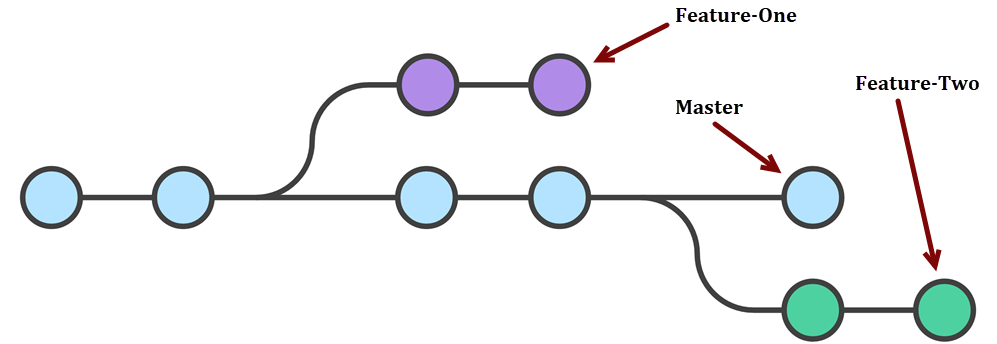
\includegraphics[width=\textwidth]{vcs-history}
\end{center}

\end{frame}


% \begin{frame}[fragile]{Version Control: merge - fast forward}
%
% \begin{center}
% 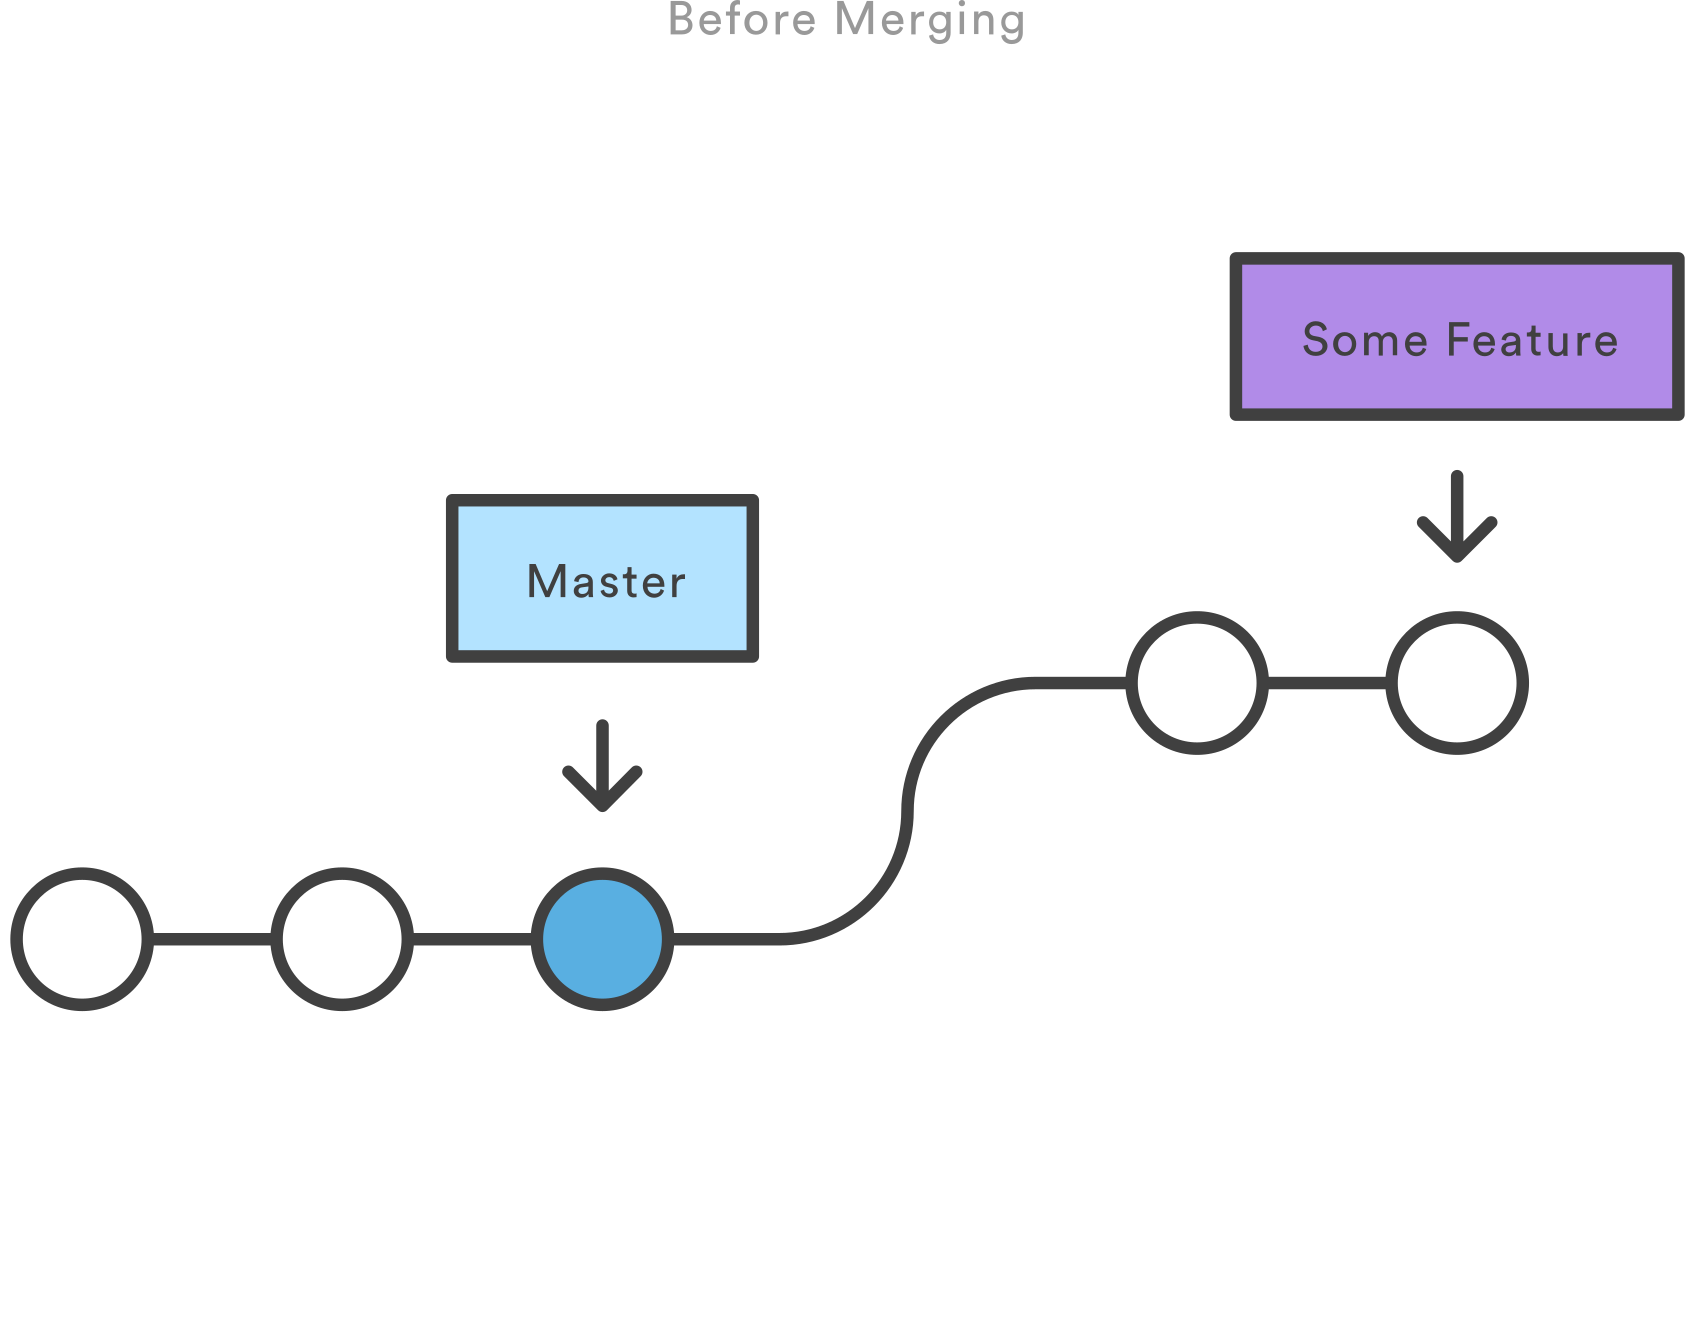
\includegraphics[width=\textwidth]{git-merge-ff}
% \end{center}
%
% \end{frame}
%
%
% \begin{frame}[fragile]{Version Control: - fast forward}
%
% \begin{center}
% 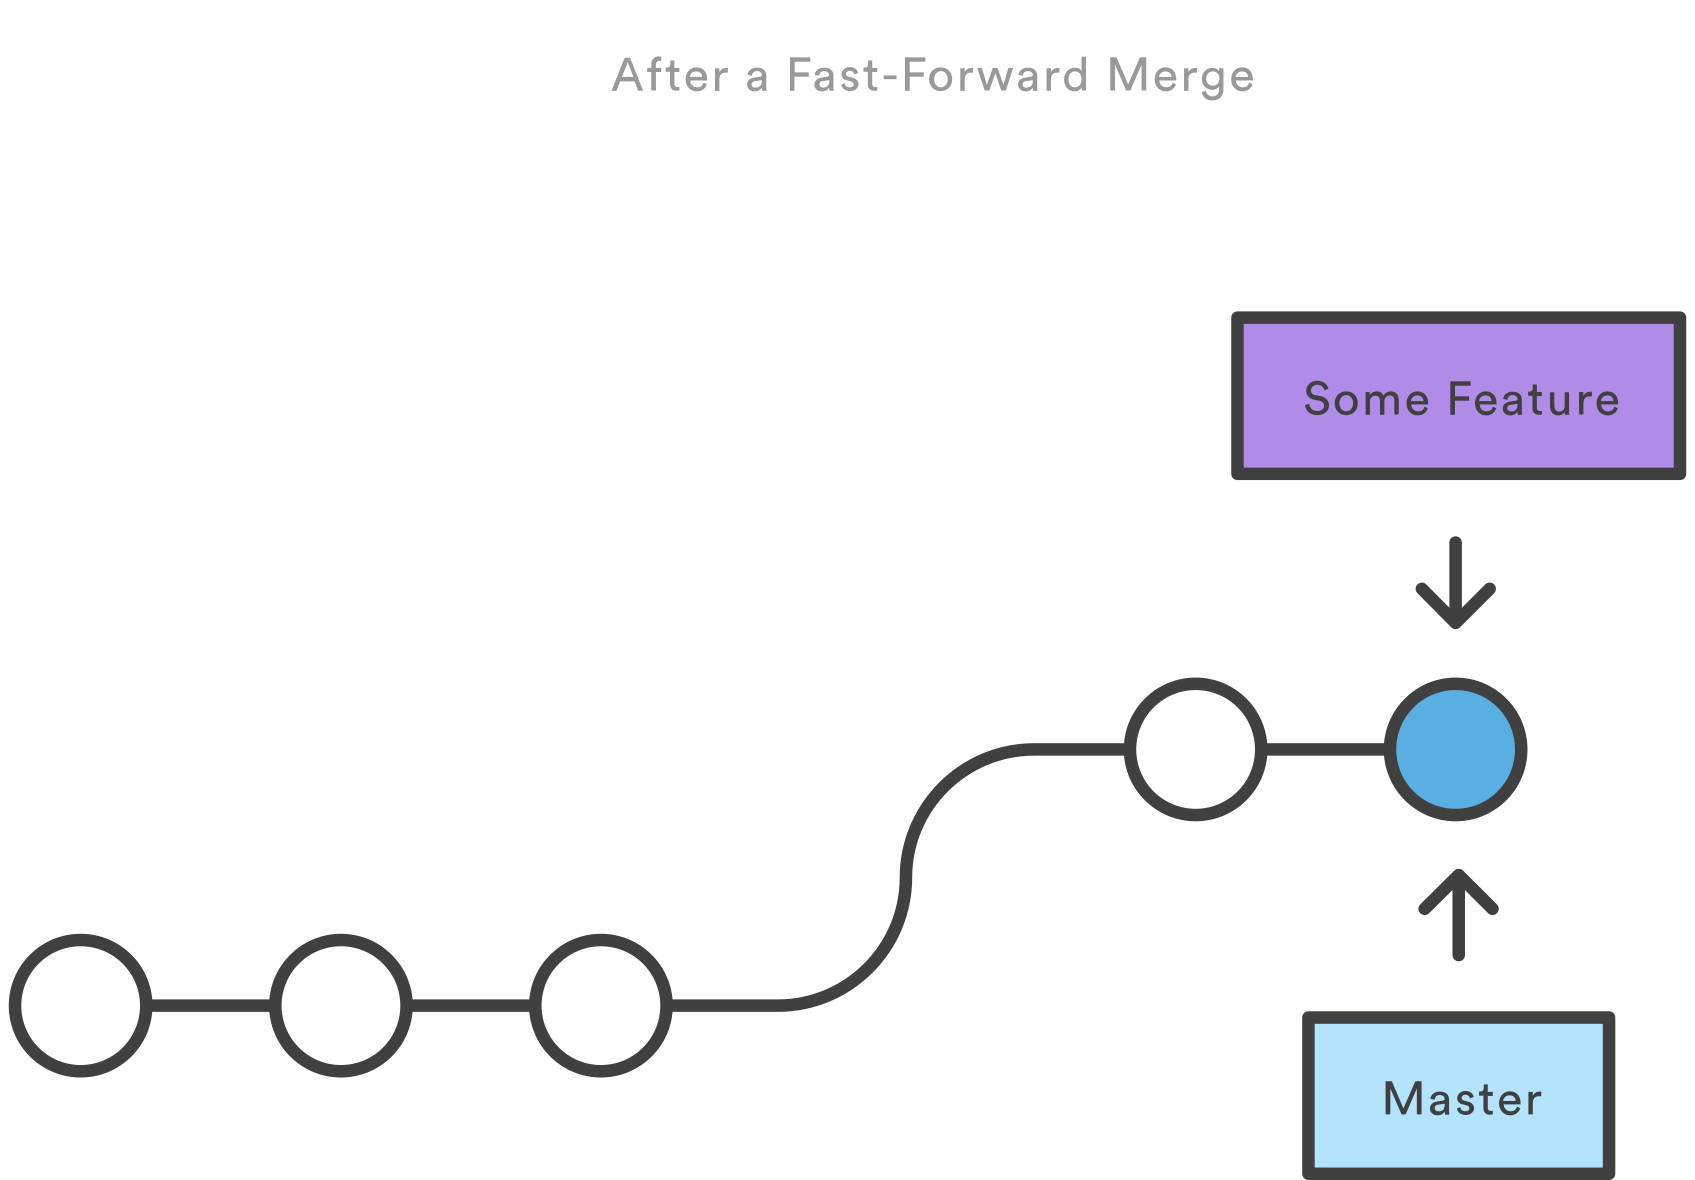
\includegraphics[width=\textwidth]{git-merge-ff2}
% \end{center}
%
% \end{frame}


\begin{frame}[fragile]{Version Control: merge - classic}

\begin{center}
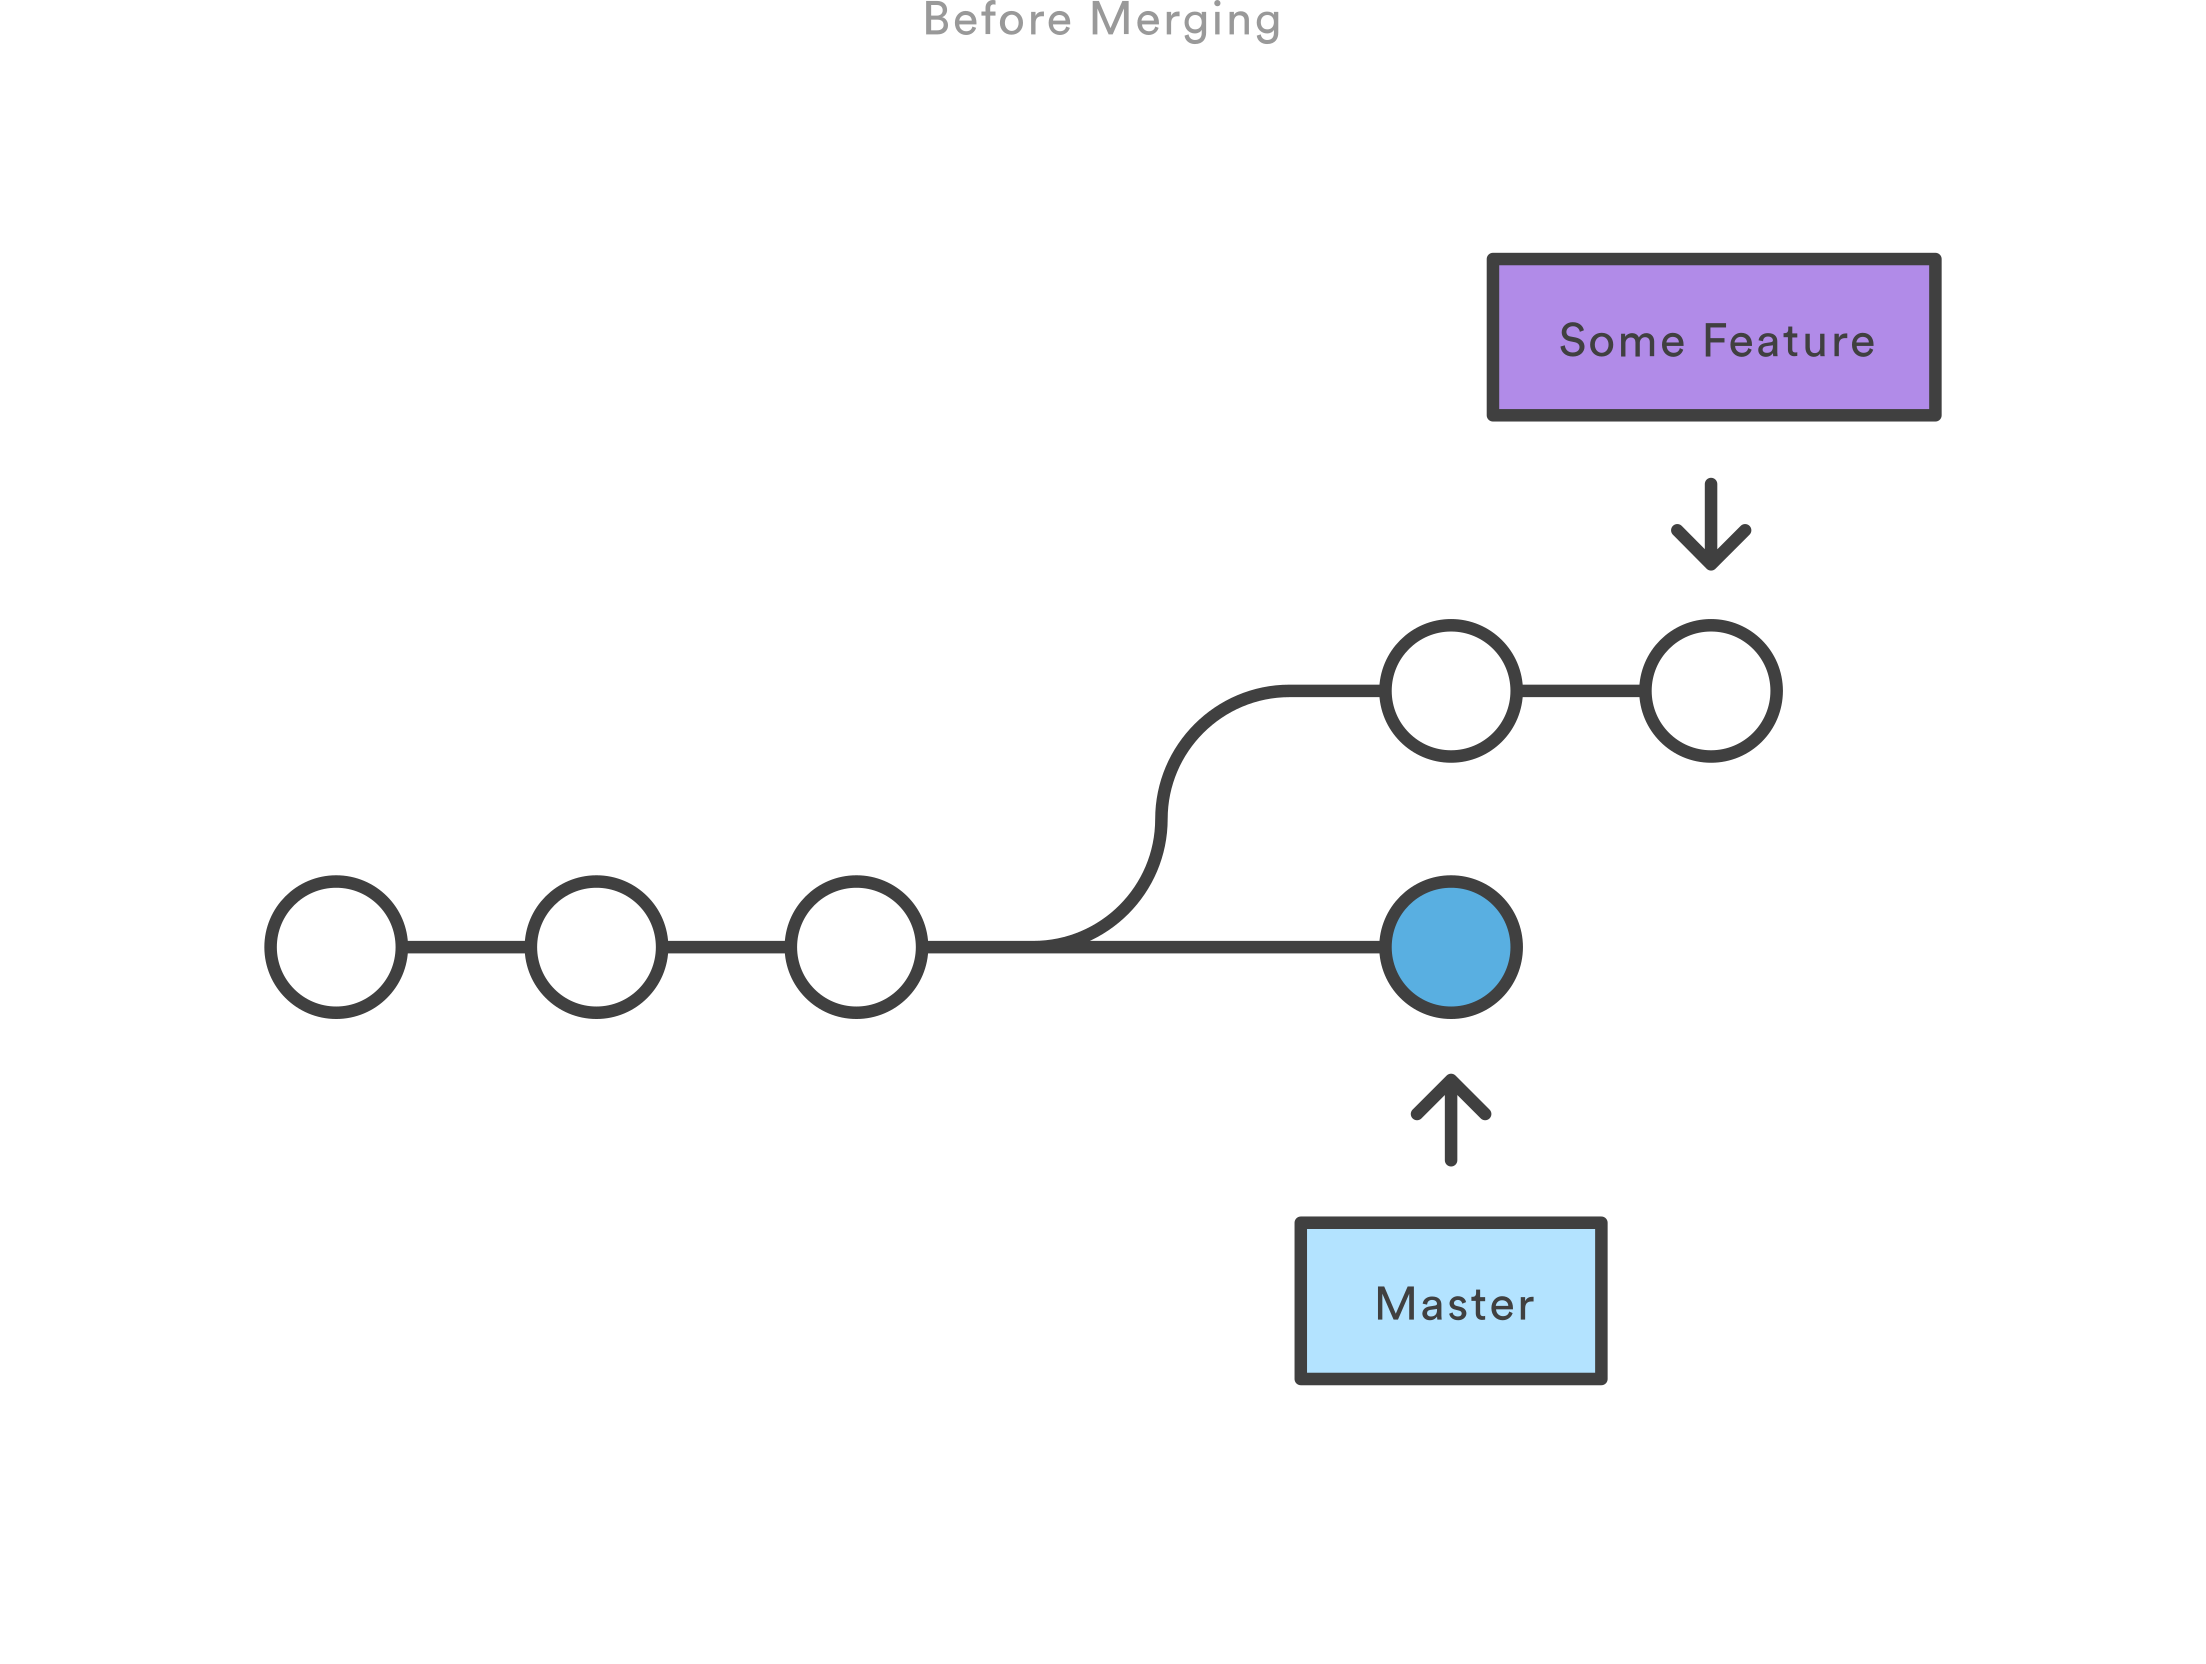
\includegraphics[width=\textwidth]{git-merge-nff}
\end{center}

\end{frame}

\begin{frame}[fragile]{Version Control: merge - classic}

\begin{center}
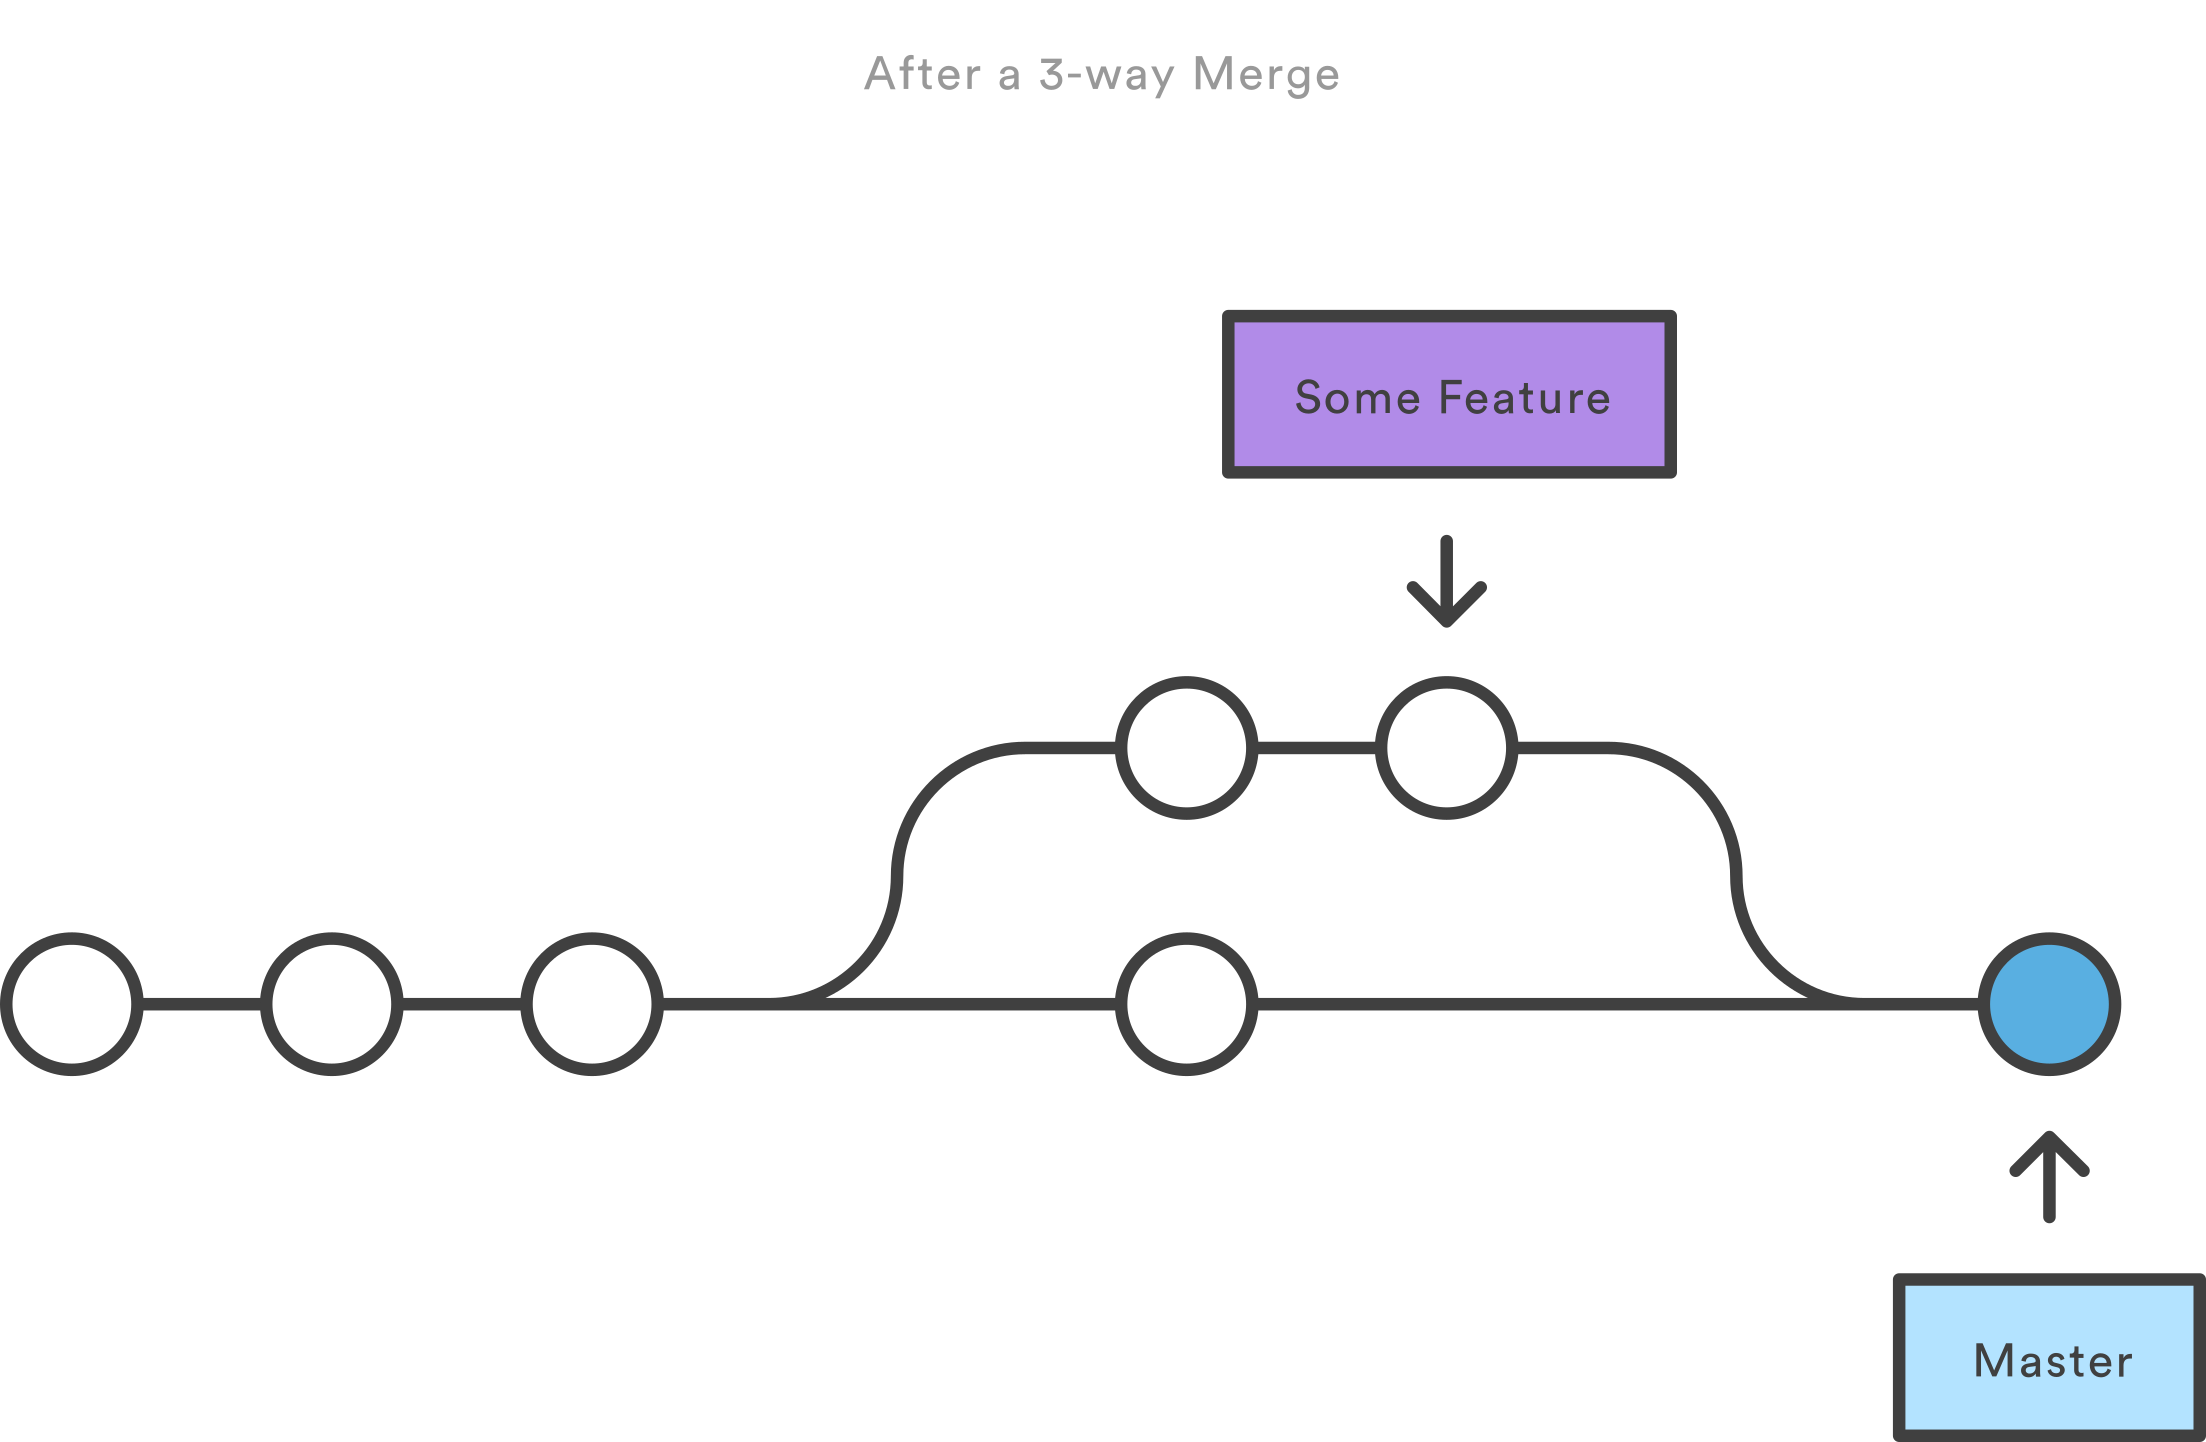
\includegraphics[width=\textwidth]{git-merge-nff2}
\end{center}

\end{frame}


\begin{frame}[fragile]{Traditional versus Distributed Version Control}

\begin{center}
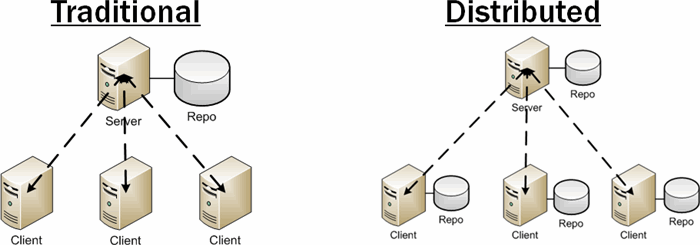
\includegraphics[width=0.7\textwidth]{vc-centralized-distributed}
\end{center}

\begin{columns}
\begin{column}{0.5\textwidth}
   \textbf{Traditional} (centralized)

   Everything lives in one place: the server. Easy to manage permissions,
     but it's not very flexible: single point of failure, clients needs to be
     constantly connected to the server, etc.
\end{column}
\begin{column}{0.5\textwidth}
  \textbf{Distributed}

  Each client has an entire copy of the repository. No single point of failure,
  no need of persistent links.
\end{column}
\end{columns}

\end{frame}




\begin{frame}[fragile]{Version control: hosting services}
\begin{itemize}
  \item Enables multiple git instances synchronization
  \item Provide ticketing systems (bugtracking/issue reporting system), project
  management, wiki for documentations
  \item Manage forks and pull requests
  \item ACL and fine granted access
\end{itemize}
\end{frame}


\begin{frame}[fragile]{Version control: well-known hosting services}


\begin{columns}
\begin{column}{0.5\textwidth}
  \begin{center}
  
\includegraphics[width=10em]{github-logo}

  
\includegraphics[width=5em]{gitlab-logo}

  
\includegraphics[width=10em]{bitbucket-logo}
  \end{center}
\end{column}
\begin{column}{0.5\textwidth}
  \begin{itemize}
    \item Most used public/private repository hosting platforms
    \item Many open source software are hosted in these services
    \item Mainly zero-cost for Open Source / Free Software, paid plans for private repositories
    \item Wiki, issues, pull requests
    \item Integrated Continuous integration and Continuous delivery
  \end{itemize}
\end{column}
\end{columns}

\end{frame}


\section{Git primitives}

\begin{frame}[fragile]{Initialize a git repository}

If we don't have a repository, we need to create it:

\vspace{2em}

\Large \texttt{git init}

\vspace{2em}

\normalsize
\begin{itemize}
  \item Git will create a new (local) repository
  \item A special directory, named \texttt{.git}, is created on the root of the
  project
  \item No file will be added to the repository
\end{itemize}

\end{frame}


\begin{frame}[fragile]{Clone an existing repository}

If a repository exists on a remote endpoint, we can clone it:

\vspace{2em}

\Large \texttt{git clone} \textit{<url>} \textit{[<localdir>]}

\vspace{2em}

\end{frame}


\begin{frame}[fragile]{Adding a file into a repository}

\vspace{2em}

\Large \texttt{git add} \textit{<file>}

\vspace{2em}

\normalsize
Adding a file into a repository means that Git will track the changes on file
contents, attributes and other metadatas.

You need to add a file into the repository both the first time (to inform Git that
you want to track that file) and before every commit where you want to ``save"
the file change (to inform Git that you want to store the change in this commit).

\end{frame}


\begin{frame}[fragile]{Create a commit in Git history}

\vspace{2em}

\Large \texttt{git commit}

\vspace{2em}

Note: if you don't specify the commit message with \texttt{-m} parameter,
Git will open the default editor to write one.

\end{frame}


\begin{frame}[fragile]{Common operations}

Create a new branch \\
\texttt{git branch} \textit{<branchname>}

Create a new branch and switch to it \\
\texttt{git checkout -b} \textit{<branchname>}

Merge the branch \textit{bob} into \textit{master} \\
\texttt{git merge} \textit{bob}

Send commits to (default) remote endpoint \\
\texttt{git push}

Retrieve commits from (default) remote endpoint \\
\texttt{git pull}

\end{frame}




\section{Git: let's use it}

\begin{frame}[fragile]{Git hosting services}
\begin{itemize}
  \item Enables multiple git instances synchronization
  \item Provide ticketing systems (bugtracking/issue reporting system), project
  management, wiki for documentations
  \item Manage forks and pull requests
  \item ACL and fine granted access
\end{itemize}
\end{frame}


\begin{frame}[fragile]{GitHub}


\includegraphics[width=10em]{github-logo}

\begin{itemize}
  \item Most used public/private git hosting platform
  \item \texttt{GNU/Linux} and many open source software are hosted into GitHub
  \item Free for Open Source / Free Software, paid plans for private repositories
  \item Wiki, issues, pull requests and so on
  \item[] \url{https://github.com/}
\end{itemize}
\end{frame}


\begin{frame}[c,fragile]{Before we begin}

On a new computer/user profile, we need to setup our environment:

\begin{center}
\begin{minipage}{\textwidth}

\begin{listing}[H]
%\scriptsize
\begin{minted}[mathescape,
							 numbersep=5pt,
							 gobble=0,
							 frame=lines,
							 framesep=2mm]{bash}
$ git config --global user.name "John Doe"
$ git config --global user.email john@doe.com
\end{minted}
\end{listing}

\end{minipage}
\end{center}

\end{frame}


\begin{frame}[c,fragile]{Start to develop on an existing Git repository}

\begin{center}
\begin{minipage}{\textwidth}

\begin{listing}[H]
%\scriptsize
\begin{minted}[mathescape,
							 numbersep=5pt,
							 gobble=0,
							 frame=lines,
							 framesep=2mm]{bash}
$ git clone https://githosting/gitrepo gitrepodir
$ cd gitrepodir/
\end{minted}
\end{listing}

\end{minipage}
\end{center}

\end{frame}


\begin{frame}[c,fragile]{Import a project into a repository}

\begin{center}
\begin{minipage}{\textwidth}

\begin{listing}[H]
%\scriptsize
\begin{minted}[mathescape,
							 numbersep=5pt,
							 gobble=0,
							 frame=lines,
							 framesep=2mm]{bash}
$ cd existingproject/
$ git init
$ git add .
$ git commit
$ git remote add origin https://githosting/gitrepo
$ git push -u origin master
\end{minted}
\end{listing}

\end{minipage}
\end{center}

\end{frame}



\section{Git: workstation setup}

\begin{frame}[c,fragile]{Before we begin}

On a new computer/user profile, we need to setup our environment:

\begin{center}
\begin{minipage}{\textwidth}

\begin{listing}[H]
%\scriptsize
\begin{minted}[mathescape,
							 numbersep=5pt,
							 gobble=0,
							 frame=lines,
							 framesep=2mm]{bash}
$ git config --global user.name "John Doe"
$ git config --global user.email john@doe.com
\end{minted}
\end{listing}

\end{minipage}
\end{center}

\end{frame}


\begin{frame}[c,fragile]{Start to develop on an existing Git repository}

If you(/your team) have an existing project on Git, you can start by \textit{cloning}
the repository locally

\begin{center}
\begin{minipage}{\textwidth}

\begin{listing}[H]
%\scriptsize
\begin{minted}[mathescape,
							 numbersep=5pt,
							 gobble=0,
							 frame=lines,
							 framesep=2mm]{bash}
$ git clone https://githosting/gitrepo gitrepodir
$ cd gitrepodir/
\end{minted}
\end{listing}

\end{minipage}
\end{center}

\end{frame}


\begin{frame}[c,fragile]{Import an existing project into a repository}

If you have an existing project outside Git, you can import it with:

\begin{center}
\begin{minipage}{\textwidth}

\begin{listing}[H]
%\scriptsize
\begin{minted}[mathescape,
							 numbersep=5pt,
							 gobble=0,
							 frame=lines,
							 framesep=2mm]{bash}
$ cd existingproject/
$ git init
$ git add .
$ git commit
$ git remote add origin https://githosting/gitrepo
$ git push -u origin master
\end{minted}
\end{listing}

\end{minipage}
\end{center}

\end{frame}




\section{Git: daily workflow}

\begin{frame}[c,fragile]{Pulling remote changes}

At the beginning of the day, or when someone push changes to server, you need to
update your local copy:

\begin{center}
\begin{minipage}{\textwidth}

\begin{listing}[H]
%\scriptsize
\begin{minted}[mathescape,
							 numbersep=5pt,
							 gobble=0,
							 frame=lines,
							 framesep=2mm]{bash}
$ cd existingproject/
$ git pull
\end{minted}
\end{listing}

\end{minipage}
\end{center}

\end{frame}


\begin{frame}[c,fragile]{Creating branch}

When needed, you can create a new branch, starting from the current commit:

\begin{center}
\begin{minipage}{\textwidth}

\begin{listing}[H]
%\scriptsize
\begin{minted}[mathescape,
							 numbersep=5pt,
							 gobble=0,
							 frame=lines,
							 framesep=2mm]{bash}
$ cd existingproject/
$ git branch new-feature-1
$ git checkout new-feature-1
$
\end{minted}
\end{listing}

\end{minipage}
\end{center}

\end{frame}


\begin{frame}[c,fragile]{Merging branch}

Let's suppose that we're on \texttt{master} branch and we want to merge \texttt{new-feature-1}

\begin{center}
\begin{minipage}{\textwidth}

\begin{listing}[H]
%\scriptsize
\begin{minted}[mathescape,
							 numbersep=5pt,
							 gobble=0,
							 frame=lines,
							 framesep=2mm]{bash}
$ cd existingproject/
$ git merge new-feature-1
$ git push
$
\end{minted}
\end{listing}

\end{minipage}
\end{center}

\end{frame}


\begin{frame}[c,fragile]{Commit and push after work}

At the end of the day, or when needed, we can create a commit by issuing:

\begin{center}
\begin{minipage}{\textwidth}

\begin{listing}[H]
%\scriptsize
\begin{minted}[mathescape,
							 numbersep=5pt,
							 gobble=0,
							 frame=lines,
							 framesep=2mm]{bash}
$ cd existingproject/
$ git add modifiedfile1 addedfile2 removedfile3
$ git commit
$ git push
\end{minted}
\end{listing}

\end{minipage}
\end{center}

\end{frame}


\begin{frame}{Useful readings}

\begin{itemize}
  \item \url{https://www.atlassian.com/git/tutorials}
  \item \url{https://git-scm.com/book/en/v2}
  \item \url{http://thepilcrow.net/explaining-basic-concepts-git-and-github/}
\end{itemize}

\end{frame}

\begin{frame}[standout]
  Questions?
\end{frame}

\begin{frame}{}

  \begin{center}\ccbysa\end{center}

\end{frame}

\end{document}
